\section{Appendix A}

08/12/2104 - this content will be added to subsequent drafts, deposited at:
http://bit.ly/1ropvH6


\section{Appendix B}

\textit{In this Appendix are an initial analysis of four frameworks: the Institutional
Analysis and Development framework from Elinor Ostrom; the Constructed
Cultural Commons framework by Madison, Frischmann and Strandburg, the
Sociotechnical Interaction Network by Kling, McKim and King, and the
Multi-dimensional In-depth Longitudinal Case Study framework by
Schneiderman and Plaisant.}
\\
\subsection*{The IAD}

In the late 1980's, the
Bloomington school began to develop a more formal framework for studying
the evolution and function of commons. The Institutional Analysis and
Development (IAD) framework was to guide the analysis of data collected
through many different empirical methods. Various versions of this
framework can be found in the work of Kiser and Ostrom \citeyearpar{kiser2000three}, Ostrom
\citeyearpar{ostrom1990governing}, Ostrom, Gardner, and Walker \citeyearoar{ostrom1994rules}, and McGinnis \citeyearpar{mcginnis2011introduction}. The settings for much of this work
were institutions that operated with a mix of governance structures, and
had a need for longevity or sustainability of a single shared resource.
Initially the IAD was designed as method-agnostic tool that could
``simplify the analytical task confronting anyone trying to understand
institutions in their full complexity.'' \citeyearpar{mcginnis2011introduction}.\\ 

Another goal of this unifying framework was to integrate the work of sociologists,
lawyers, politicians, economists, and political scientists in trying to
understand how ``institutions affect the incentives confronting
individuals and their resultant behavior'' \citep{ostrom2009understanding}. While the
original goal may have been to simplify the task of studying
institutions in diverse settings, the IAD has been used, adapted and
modified so many times that it often seems incomprehensible as a single
framework. Below, I sketch out the most basic features of the
framework.The IAD divides an investigation into three levels of analysis
for studying ``underlying factors'' of an intsituion's success or
failure -- (1) exogenous variables, (2) action arenas, and (3) outcomes
and evaluations.\\

\begin{enumerate}
\item 
1. Exogenous variables include biophysical attributes of
the shared resources, community attributes, and structural governance
policies (formal or informal).Exogenous variables are also considered
the ``input'' to a complex system.\\ 
\end{enumerate}

In his overview of the framework
Frischmann gives a simple example of this group, from the Maine Lobster
fishing grounds, "\ldots{}attributes might include the relevant
biological characteristics of lobsters, such as the rates at which they
age and reproduce; attributes of the community of fishermen, such as the
proximity in which they live to others, the existence of familial
relationships, and the skill sets needed for lobster fishing; and the
rules---explicit or informal---that govern fishing." \citep{frischmann2013two}. The most crucial aspect of this level is that while individual
attributes or variables are identifiable and observable, they need not
be considered fully decomposable \citep{ostrom2009understanding} -- meaning that the
salient features of a commons are often thought to be ``emergent
properties'' where the mutual constitution of people and objects (in the
case of ICOADS technologies) create phenomena which are indivisible. The
use of multiple research methods for the same institutional setting are
often justified on the grounds of needing to understand these emergent
properties \citep{ostrom2009understanding}.\\

\begin{enumerate}
\item
2. An Action Arena -- space where exogenous
variables and actors interact, cooperate, and conflicts emerge. This level
of the IAD places the stakeholders and the resources of the commons --
as inventoried in level 1 -- into a particular setting such as the
harvest of a shared common field. Using the understanding gained from
level one, the analyst observes this process and then identifies
tangible outcomes, objective results and the way that conflicts from the
past, or the present are voiced, contested, settled or deferred. This
analysis can take place over long periods of time, to give a
longitudinal account of action such as the restoration of an aquifer
\citep{ostrom2010moving} or a statistical analysis of these processes
through agent-based models or multi-modal network analysis \citep{axelrod1997advancing}.\\
\end{enumerate}
\begin{enumerate}
\item
3. Outcomes and Evaluation -- the results and feedback of action
situations In the final stage of the framework an institution can be
evaluated based on outcomes of the action arena; that is, how well an
institution did or did not solve a collective action problem. Criteria
for evaluation will vary by institutional setting, but usually includes
calculation of transaction costs, such as (1) information costs (2)
coordination costs; and, (3) strategic costs, or
sustainability of the shared resource in terms of (1) efficiency in
access and use (2) equity of distributed wealth or costs, (3)
accountability for resource management, or (4) adaptability of the
institution in light of these outcomes  \citep{imperial2005taking}.\\ 
\end{enumerate}

\begin{figure}
\centering
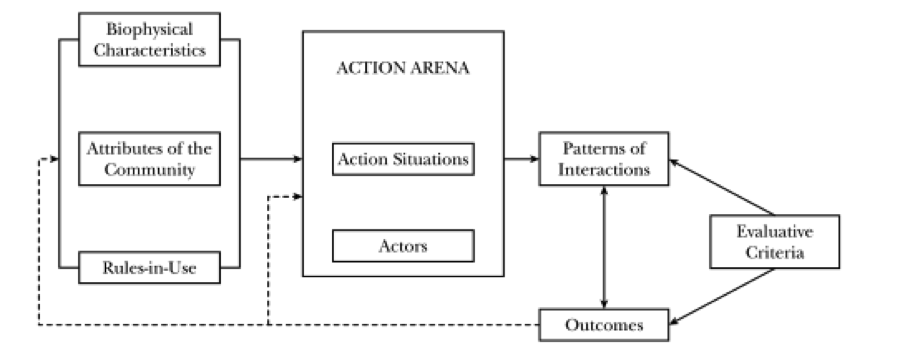
\includegraphics[width=\textwidth]{Ost}
\caption{The framework of the IAD (Ostrom, 2005, p.~15)}
\label{fig:my_label}
\end{figure}

For commons made up of natural resources, of the
type previously studied by institutional scholars: the boundaries were clear,  the resource systems studied were small and easy to observe, solving problems was of high salience to appropriators, institutions were long-enduring and had evolved over time, and (5)
extensive field observation was available \citep{ostrom2011background} Each of these
assumptions is complicated, if not completely opposite for peer produced
commons of digital material. Notably, boundaries are unclear, resource
systems (commons) are large, distributed and impossible to observe
qualitatively, and institutions are rapidly evolving- often existing for
short funding cycles that are of the 5-10 year range. While the IAD
provides a starting point, the dynamic nature of purposefully built
commons of digital objects requires much more innovation than a simple
re-tooling of terminology \citep{hess2007understanding}. In the next section I
review a proposal for the constructed cultural commons, which provides a
novel way to overcome some of these limitations.\\ 

\subsection*{Constructed Cultural Commons} 

In a broad ranging discussion of the purely functional
account of common property regimes, three lawyers - Maddisson,
Frischmann and Strandburg , propose a new framework for studying the
cooperative work of cultural institutions facing collective action
problems. In this account, ``constructed cultural commons,'' are defined
as, ``environments for developing and distributing cultural and
scientific knowledge through institutions that support pooling and
sharing of that knowledge in a managed way'' \citep[p. 659]{madison2010constructing}. Constructed cultural commons are, as MFS
explain, markedly different than the natural resource commons of Ostrom
et al's study, ``These environments are designed and managed with
limitations tailored to the character of those resources and the
communities involved rather than left to evolve via market transactions
grounded solely in traditional proprietary rights'' \citep[p. 659]{madison2010constructing}\\

Madison, Frischmann and Strandburg propose that in creating a unified
framework for studying the success and failures of diverse cultural
commons by aligning their ``social role and significance'' within nested
institutions. In particular, their framework is to be used for works of
pooled resources that are not subject to the same types of intellectual
property laws that govern private property or common-pool resources.
MFS's proposal does not suggest moving away from functionalism, but to
add to it through a form of `analytical narrative' \citep{bates2000analytical},
where ``In proper proportion, a humanistic and metaphorical inquiry into
information policy, on one hand, and a functional approach grounded in
social science models, on the other hand'' \citep[p. 673]{madison2010constructing}. Or in other
words, a unified framework that can account for new modes of knowledge
production, distribution and the purposeful construction of cultural
objects in physical and digital forms.\\

Their proposed framework achieves
this through three major innovations with the IAD: 1. It emphasizes among
distributed actors, and the constructed nature of the resources
themselves (purposefully built objects as opposed to natural
resources) 2. Where the IAD separates ``outcomes'' (level 2) and
``patterns of interactions'' (level 3) the constructed cultural commons
framework treats these as iterative, mutually constitutive processes. 3.
As a result of the more complex relationships between resources,
participants, and governance structures-- the ``relevant'' attributes of
each may not neatly divide into categories.\\ 

\begin{figure}
\centering
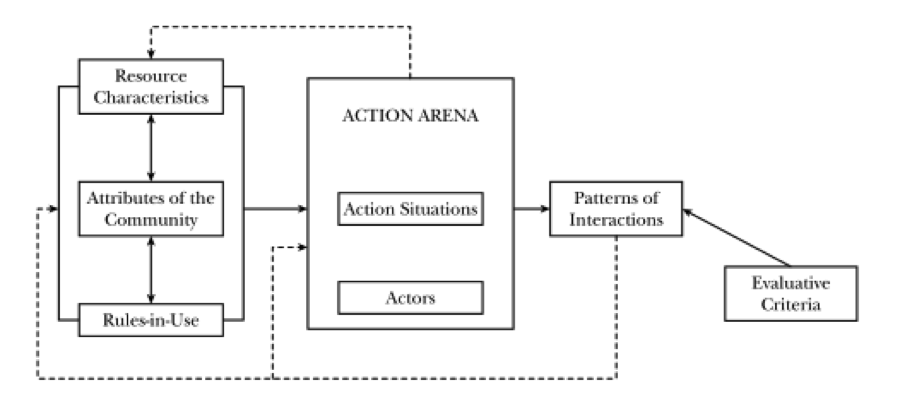
\includegraphics[width=\textwidth]{Mad}
\caption{Madison, Frischman and Strandburg's modification the IAD for a Constructed Cultural Commons \citep{madison2010constructing}}
\label{fig:my_label}
\end{figure}

In short, this is the acknowledgment of a ``mutually constitutive'' sociotechnical
perspective.This innovation with IAD is therefore particularly useful
for studying public goods, which do not fit cleanly into private or
cooperatively owned property regimes. The quintessential case for
constructed cultural commons are free and open source software projects
such as Apache or Linux, but the authors note that the ambition of their
framework is to include a diverse set of constructed commons such as the
case studies they offer on patent pools amongst technology firms.\\
\\

\subsection*{Sociotechnical Interaction Networks (STIN)} 

The socio-technical interaction network is a framework published late in Rob Kling's life, producing only two publications that described its features through use cases having to do with scholarly communications \citep{kling2000scientific, kling2003bit}. A broader definition in the second of these publications was that a STIN would be a, ``conceptual framework for identifying,
organizing, and comparatively analyzing patterns of social interaction,
system development, and the configuration of components that constitute
an information system'' (Kling, McKim and King, 2003).\\

STIN was heavily influenced by actor-network
theory in that the elements of a network are not treated as decomposable
entities, but instead studied for the strength or weakness of their
associations (i.e.~Latour's dictum that ``nothing can be reduced to
anything else, nothing can be deduced from anything else, everything may
be allied to everything else'' (1988, p.~163)) is analogous to the
``co-constitution'' of the social and technical network that studies
associations. The difference being that while Latour hopes to give an
account of a specific moment in which a network of associations achieves
(or fails) Kling is interested in the shaping of communication systems,
and the purposeful design and engineering of associations within those
systems. Another way to put the difference is that where Latour asks
``What's going on here, really?'' in the metaphysical sense, Kling asks,
``What's supposed to go on, what do we want to go on, and how can we
design a system to facilitate this?'' in the normative sense. The former
is concerned with creating an object-oriented ontology to be put to use
by sociologists of associations (Harman, 2003; Latour, 2005), where the
latter is, like the cyberneticists stating that ``What can be studied is
always a relationship or an infinite regress of relationships. Never a
`thing'\,'' (Bateson, 2000).\\

Some assumptions that STIN and the socio-technical approach more
generally accept are the following:

\begin{enumerate}
\def\labelenumi{\arabic{enumi}.}
\item
  The social and technical are not meaningfully separable. This is the
  very idea of a mutual constitution between these two elements.
\item
  Theories of social behavior can and should influence technological
  design choices (STIN has a normative dimension)
\item
  Actors are embedded in multiple social relationships, only some of
  which are technologically mediated. Being a part of many networks,
  people may have conflicting commitments. An STS plays differing roles
  in the lives (professional, educational, etc) of an actor.
\item
  Sustainability and routine operations are critical and must play a
  role in determining design.
\end{enumerate}

STIN has rarely been adopted, but is often cited for its potential to
guide or inform work of a sociotechnical concern (Myer, 2006). Studies
where the framework has been used include Web Implementation Systems
(Eschenfelder and Chase, 2005), Digital Libraries (Rosenbaum, 2007), and teams of
Open Source Software development systems (Scacchi, 2005).

\textbf{Modeling a STIN}

In Kling, McKim and King's study of collaboratories they outline the
following steps, noting that these are to be seen as "illustrative rather
than enumerative" (2003).\\

\begin{itemize}
\itemsep1pt\parskip0pt\parsep0pt
\item
  Identify a relevant population of system inter-actors
\end{itemize}

This is very similar to a traditional ``stakeholder analysis'' in
systems development. STIN researchers attempt to understand the
diversity of actors, their roles, and their needs with respect to the
system being studied

\begin{itemize}
\itemsep1pt\parskip0pt\parsep0pt
\item
  Identify core ``inter-actor'' groups
\end{itemize}

Uses results of first step to group actors - also, attempts to make
clear the conflicts that may emerge between groups and between
individuals that may be a part of many groups.

\begin{itemize}
\itemsep1pt\parskip0pt\parsep0pt
\item
  Identify incentives
\end{itemize}

Kling et al. describe this as the ``business model'' of a STIN- asking
``what would energize appropriate communication in the forum'' of a
scholarly communication system. Understanding the ways and means of
sustaining that energy may be explained by a theory of social
interaction explicitly, or implicitly.

\begin{itemize}
\itemsep1pt\parskip0pt\parsep0pt
\item
  Identify excluded actors and undesired interactions
\end{itemize}

Understanding the sustainability of a STIN also depends on modeling what
interactions, and what forms of interactions that actors do not want.

\begin{itemize}
\itemsep1pt\parskip0pt\parsep0pt
\item
  Identify existing communication forums
\end{itemize}

This step is an attempt to characterize an actor (or group of actors)
``communication ecology'' . Kling et al. also instruct that this should
be done with particular attention paid to how or why a new design might
introduce competition in this ecology.

\begin{itemize}
\itemsep1pt\parskip0pt\parsep0pt
\item
  Identify resource flows
\end{itemize}

In short, this is described as a ``follow the money'' exercise to track
resources throughout a STIN.

\begin{itemize}
\itemsep1pt\parskip0pt\parsep0pt
\item
  Identify system architectural choice points
\end{itemize}

After characterizing the STIN, this model proposes to identify system
architectures and their ``choice points'', which refer to ``a
technological feature or social arrangement in which the designer can
select alternatives''

\begin{itemize}
\itemsep1pt\parskip0pt\parsep0pt
\item
  Map architectural choice points to socio-technical characteristics
\end{itemize}

This process combines all steps in proposing ``combinations and
configurations of features that are most compatible, viable, and
sustainable.'' (Kling, McKim and King, 2003 p.~57)

\subsection*{Multidimensional In-Depth Long-term Case Studies (MILC)}

The last framework to be evaluated comes from the field of human
computer interaction (HCI). Although this framework does not deal with
sustainability per se, it is included for the following reasons:\\

\begin{itemize}
\itemsep1pt\parskip0pt\parsep0pt
\item
  MILC's are used to study action situations over long periods of time.
  Thus, it provides insight as to how a framework might deal with
  longitudinal events, such as sustainable practices in a data archive.
\item
  By focusing on design scenarios which are ``situated'' and highly
  responsive to contextual factors, the MILC framework offers a way to
  integrate sociotechnical scholarship which is incompatible with much
  of the IAD's functionalism.
\item
  MILC's have a unit of analysis that is constructed, built, or
  purposefully engineered - as such, the framework is concerned not with
  simply cataloguing the existence of an object over time, but improving
  its features and performance along the way.
\item
  Like STINs, a MILC has a normative dimension, but this framework
  includes a consideration of interventions that are design-oriented.
\end{itemize}

Schneiderman and Plaisant describe the ``Multi-dimensional In-depth
Long-term Case studies'' by way of deconstructing its various terms \citep{shneiderman2006strategies}:

\begin{itemize}
\itemsep1pt\parskip0pt\parsep0pt
\item
  \textbf{Multi-dimensional} refers to using observations, interviews,
  surveys, as well as automated logging to assess user performance
  interface efficacy, and utility.
\item
  \textbf{In-depth} refers to the intense engagement of the researchers
  with the expert users to the point of becoming a partner or assistant.
\item
  \textbf{Long-term} refers to longitudinal studies that begin with
  training in use of a specific tool through proficient usage that leads
  to strategy changes for the expert users.
\item
  \textbf{Case studies} refers to the detailed reporting about a small
  number of individuals working on their own problems, in their normal
  environment (2006, p.1).
\end{itemize}

The outcomes of a MILC usually take two forms:

\begin{enumerate}
\def\labelenumi{\arabic{enumi}.}
\item
  The refinement of the tool and an understanding of general principles
  or guidelines for the design of such tools.
\item
  The achievement of the expert users' goals, by way of their gaining
  some form of mastery over the tool.
\end{enumerate}

Use of the MILC framework is limited by the need to have willing
participants, and a stable field of study for long periods of time. As
reported by Valiati, Freitas, and Pimenta in their use of MILC during a
project that took twice as long as they had scheduled for completing a
single case study, ``performing multiple longitudinal case studies in a
parallel way is a very hard task, due the difficulty of finding users to
participate and the availability of the users during the study'' (2008).\\